\section{Evaluation}
\label{sec:evaluation}

\subsection{Experimental Setup}
\paragraph{Hardware and execution}
All experiments run on one instance configuration: an Intel Xeon Platinum 8352V with a 32-CPU allocation, a 60 GiB memory limit, and a 56 GiB process-family guard. Query throughput is measured at 1, 8, 16, and 32 threads with fixed CPU affinity. Every index builder is configured with eight threads; Lucene adds documents serially before its eight-thread merge, and a separate experiment varies QuIVer's construction threads. Builds, timed queries, compilation, and large transfers are serialized to avoid interference. Supplementary experiments build their own indices from the same inputs and frozen configurations; their throughput and build times are compared only within each experiment.

QuIVer is compiled in release mode with native CPU targeting, link-time optimization, and one code-generation unit; the C++ wrappers we compile for SymphonyQG, HNSWlib, and VSAG use \texttt{-O3 -march=native}, and RaBitQ keeps its official SIMD dispatch. The query benchmark calls the integrated QuIVer kernel with the database's vector-pool callback. It measures ANN processing and reranking, excluding network transport, query-language parsing, and payload serialization. External methods use their native batch interfaces, with interface and timing boundaries recorded per measurement. SVS processes each query set in one call and exposes no per-request latency, so its tail latencies are unreported.

\paragraph{Datasets and splits}
Table~\ref{tab:datasets} lists all 21 datasets, including two five-million-vector collections. Three workloads have external comparisons: Cohere-1M-768, DBpedia-990K-1536, and Cohere-5M-768. The remaining datasets evaluate QuIVer's dimensionality, scale, and representation dependence. Cosine datasets are normalized, while SIFT and GIST retain native L2 distance, original magnitudes, and zero vectors. Ground truth refers to the actual evaluated database subset. In particular, truncated Arxiv, CodeSearch, and GooAQ collections use recomputed FP64 ground truth over their million-vector subsets.

Each dataset reserves 256 queries for parameter selection. The remaining 744 or 9,744 queries, depending on the dataset, form the evaluation set. The core comparisons share the same query identifiers across methods. The benchmark query collections were also used during development; in particular, all 744 Cohere evaluation queries appeared in earlier development experiments, so we also evaluate held-out queries (Sections~\ref{sec:ablation} and~\ref{sec:system}). The four-dataset mechanism experiment uses 200K subsets and independently recomputes their full ground truth. Sources include BGE-M3~\cite{chen2024bgem3}, Wolt-CLIP~\cite{woltclip2024}, and RedCaps~\cite{desai2021redcaps}.

\paragraph{Parameters and repetition}
QuIVer uses $R=64$, construction width $e_c=128$, and the selection rule in Equation~\eqref{eq:prune}. Each main dataset has one constructed graph; Section~\ref{sec:system} reports independent rebuilds. Search widths are selected from
$\{32,48,64,88,128,192,256,384,512,768,1024\}$.
For each of the 90\%, 95\%, and 98\% validation-recall targets, we select the smallest qualifying width. We retain a highest-budget point and additional widths chosen by a fixed budget-spacing rule, up to five distinct widths. Multithread measurements reuse the selected target widths. External methods retain their corresponding validation-selected construction and search configurations.

We measure five throughput rounds after warming the query working set and report their arithmetic mean. A QuIVer round lasts at least five seconds and contains complete passes over the evaluation queries. Latency is collected separately over five complete passes, measuring native service time without client queueing. P95/P99 confidence intervals resample queries as clusters, keeping their repeated measurements together. Recall is the mean fraction of the exact top ten returned. Recall--throughput evaluation follows the benchmarking perspective of ANN-Benchmarks and comparative studies~\cite{aumuller2020annbenchmarks,aumuller2023trends,li2019annanalysis}.

\paragraph{Baselines}
The comparison archive contains 30 external modes: full-precision HNSW implementations in FAISS, HNSWlib, USearch, and VSAG; DiskANN in FP32 and PQ variants; Lucene BBQ; centered and uncentered FAISS BinaryHNSW with FP32 reranking; SVS LVQ4, LVQ8, and two-level LVQ; SymphonyQG; NGT-QG; HSCG; MIRAGE-ANNS; $\alpha$-CNG; and IVF-Flat, PQ, OPQ/FastScan, and RaBitQ variants. FAISS RaBitQ with SQ8 reranking and variants with FP32 reranking are distinct modes. Original-vector use and quantized refinement remain part of each method's measured configuration.

Figure~\ref{fig:curves} shows the available single-thread curves, each joining search widths of one constructed index. Table~\ref{tab:main} reports the validation-selected 95\% configurations of nine methods, including the strongest high-throughput quantized graphs and compact alternatives, with their achieved evaluation recall.

For these configurations, SymphonyQG uses degree/beam settings 64/400 on Cohere-1M and 32/200 on the other two workloads, with three refinement iterations. Lucene BBQ uses connectivity/construction-width settings 32/400 on Cohere-1M and 16/200 on the others. SVS LVQ8 and VSAG SQ8 use degree/beam settings 32/200, with SVS padding parameter 32. HNSWlib uses $M=16$ and \texttt{efConstruction}=200. DiskANN uses degree/beam settings 32/200 on Cohere-1M and DBpedia-1536 and 64/400 on Cohere-5M. NGT-QG uses ANNG degree 40, outgoing degree 32, and quantizer parameters $Q=2$, $k=32$, $p=8$. RaBitQ IVF uses 4,096 inverted lists and \texttt{nprobe}=128 on all three workloads in Table~\ref{tab:main}, with its official 32-bit FP32-refinement mode. Complete measurements for all 30 baseline modes and QuIVer, including configurations and timing definitions, are provided in the \href{https://github.com/YoKONCy/TriviumDB/tree/master/evaluation}{evaluation archive}.

\paragraph{Measurement definitions}
$T_{\mathrm{idx}}$ is the recorded index preparation time. For QuIVer it covers graph construction and SM installation. For SymphonyQG, HNSWlib, VSAG, and RaBitQ it is the official build call, and for SVS the LVQ quantization and Vamana build calls; serialization is excluded for these methods and for QuIVer. NGT-QG's build commands include their internal persistence, Lucene's time spans insertion through forceMerge and commit, and DiskANN's includes its PQ training.

$M_{\mathrm{nav}}$ sums the persistent navigation components, including any full-precision navigation data. $M_{\mathrm{total}}$ adds the separate original-vector store used for reranking, which methods such as SymphonyQG and SVS do not need. Query-process RSS is retained in the companion measurement data.

\begin{figure*}[!t]
\centering
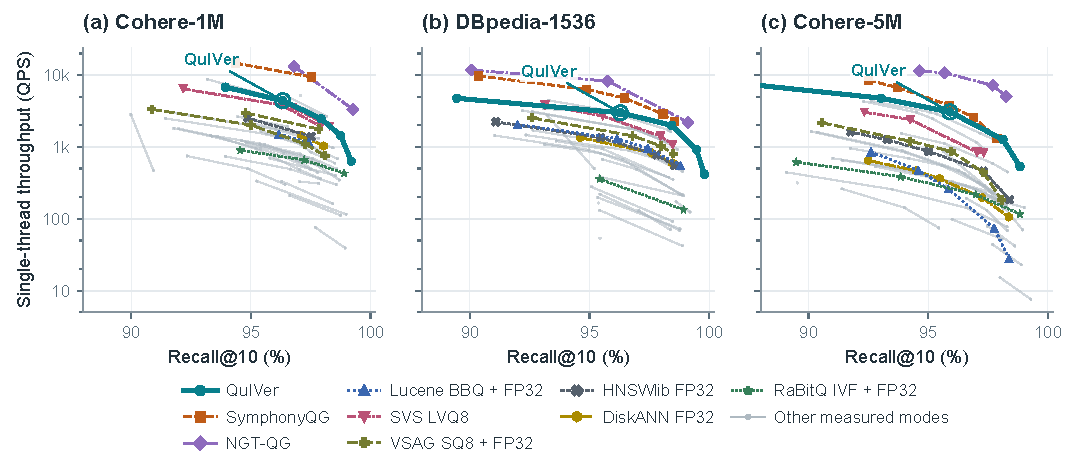
\includegraphics[width=\textwidth]{recall-throughput.pdf}
\caption{Single-thread curves at 88--100\% evaluation recall, with shared logarithmic QPS scales. Colors, markers, and line styles identify representative methods; gray traces retain other measured modes. Lines join points from the same index. Outlined QuIVer markers identify frozen validation-selected 95\% configurations; their horizontal positions show actual evaluation recall.}
\label{fig:curves}
\end{figure*}

\begin{table*}[!t]
\caption{Validation-selected 95\% operating points. Recall $r$ is the observed evaluation Recall@10; QPS values average five rounds. $T_{\mathrm{idx}}$ includes QuIVer's graph construction and SM installation. Memory columns are logical component subtotals in GiB; $M_{\mathrm{total}}-M_{\mathrm{nav}}$ is the separate original-vector store. P99 is single-thread service latency in milliseconds; \missing{} indicates unavailable native latency.}
\label{tab:main}
\centering
\footnotesize
\setlength{\tabcolsep}{3.5pt}
\begin{quivercheckedtable}{main-comparison}
\begin{tabular}{llrrrrrrrrr}
\toprule
Dataset & Method & $r$ (\%) & 1T QPS & 8T QPS & 16T QPS & 32T QPS & $T_{\mathrm{idx}}$ (s) & $M_{\mathrm{nav}}$ & $M_{\mathrm{total}}$ & P99 \\
\midrule
\tabularinput{tables/main-comparison.tex}
\bottomrule
\end{tabular}
\end{quivercheckedtable}
\end{table*}

\subsection{Pareto Efficiency across Construction, Memory, and Throughput}
\label{sec:mainresults}
QuIVer's validation-selected 95\% configurations lie on the measured Pareto frontiers of all three core workloads at both one and 32 threads. We maximize achieved recall and throughput and minimize $T_{\mathrm{idx}}$ and memory: no measured point matches or improves every dimension and improves at least one. This holds whether memory is $M_{\mathrm{total}}$, $M_{\mathrm{nav}}$, or, for points with recorded RSS, query-process RSS. The comparison uses the full measured curves, including the actual recalls of points that miss their validation targets. Figure~\ref{fig:memory} shows the cost--throughput projections.

\paragraph{Cohere-1M}
At 96.33\% recall, QuIVer reaches 4,396 single-thread QPS. Lucene BBQ reaches 1,503 QPS at 96.17\%, and SVS LVQ8 reaches 3,814 at 96.29\%. These close-recall points give throughput ratios of $2.92\times$ and $1.15\times$, respectively. QuIVer's graph build takes 89.40 s and SM installation 11.16 s. Its total logical memory is 3.781 GiB, against 3.032 GiB for BBQ and 0.868 GiB for LVQ8, whose compressed vectors need no separate store.

QuIVer uses $3.03\times$ and $2.35\times$ less total logical memory than SymphonyQG and NGT-QG ($12.44\times$ and $6.54\times$ less navigation storage), and its recorded preparation is $5.82\times$ and $16.94\times$ faster.

\paragraph{DBpedia-1536}
At 96.29\% recall, QuIVer reaches 2,987 QPS with 1.265 GiB of navigation components and 6.930 GiB in total. Lucene BBQ reaches 1,303 at 96.15\%, while SVS LVQ8 reaches 2,692 at 95.55\%. QuIVer's 128.45 s graph build and 20.83 s installation together take 149.28 s. Relative to LVQ8, this gives higher recall, $1.11\times$ throughput, and $3.44\times$ faster preparation, whereas LVQ8 needs $4.42\times$ less total memory.

Table~\ref{tab:high} reports the 98\% target configurations. QuIVer reaches 98.43\% at 1,997 QPS; LVQ8 reaches 98.47\% at 1,073 QPS, and SymphonyQG reaches 98.56\% at 2,265 QPS. At these nearby recalls, QuIVer delivers $1.86\times$ LVQ8's throughput and 88\% of SymphonyQG's throughput with $1.98\times$ less total logical memory than SymphonyQG. The corresponding query-process RSS is approximately 7.00 GiB for QuIVer, 13.85 GiB for SymphonyQG, and 1.73 GiB for LVQ8.

\paragraph{Cohere-5M}
The five-million-vector workload combines near-SymphonyQG concurrent throughput with lower memory and preparation cost. QuIVer reaches 95.90\% recall at 3,075 single-thread QPS; SymphonyQG reaches 95.87\% at 3,801 QPS. QuIVer retains 81\% of its single-thread throughput and 97\% of its 32-thread throughput (34,109 versus 35,276 QPS). Total logical memory falls from 35.763 to 18.906 GiB (47.1\%) and navigation storage to 4.601 GiB (87.1\%); preparation is $2.15\times$ faster. SymphonyQG's payload comprises 14.305 GiB of FP32 navigation vectors, 19.073 GiB of per-edge local codes, 1.788 GiB of edge factors, and 0.596 GiB of neighbor identifiers.

QuIVer also delivers $11.74\times$ Lucene BBQ's single-thread throughput at nearby recall (95.83\% for BBQ), using $1.26\times$ its 15.062 GiB total logical memory. NGT-QG reaches 10,751 QPS at 95.67\% recall with 44.441 GiB in total and a 15,774 s recorded build. QuIVer's 465.22 s graph build and 59.37 s SM installation give $30.07\times$ faster preparation and $2.35\times$ less total logical memory.

\paragraph{Uncertainty and matched recall}
Query-bootstrap 95\% intervals for QuIVer's recall are [95.34, 97.20]\%, [96.03, 96.55]\%, and [94.88, 96.87]\% on the three workloads, and its five-round single-thread throughput varies by at most 1.9\% (CV). Paired with SymphonyQG, the recall differences on DBpedia-1536 ($-0.16$ pp) and Cohere-5M ($+0.03$ pp) have intervals containing zero. Interpolating each fixed configuration's single-thread curve to 95\% recall gives QuIVer 5,599, 3,261, and 3,528 QPS. SymphonyQG reaches $2.39\times$, $1.89\times$, and $1.36\times$ these values and NGT-QG $2.65\times$ and $3.18\times$ on the last two workloads, whereas QuIVer reaches $1.25\times$, $1.12\times$, and $1.95\times$ LVQ8's. QuIVer's frontier position thus combines throughput with preparation time and memory rather than maximizing throughput alone.

\begin{figure*}[!t]
\centering
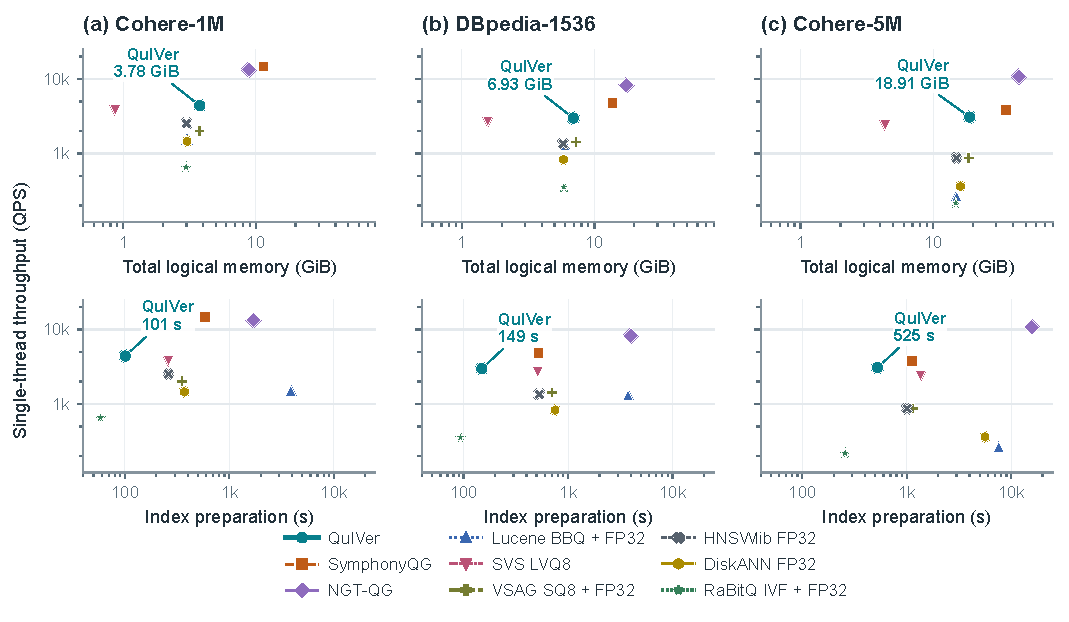
\includegraphics[width=\textwidth]{memory-throughput.pdf}
\caption{System trade-offs at the frozen configurations of Table~\ref{tab:main}: total logical memory $M_{\mathrm{total}}$ versus QPS (upper), and recorded index preparation $T_{\mathrm{idx}}$ versus QPS (lower). Logarithmic scales are shared across datasets. Upper-left positions indicate lower cost and higher throughput. The table supplies achieved recall, navigation memory, and timing definitions.}
\label{fig:memory}
\end{figure*}

\begin{table}[t]
\caption{Validation-selected 98\% configurations. Each dataset reports achieved evaluation recall (\%) and single-thread QPS.}
\label{tab:high}
\centering
\footnotesize
\setlength{\tabcolsep}{1.4pt}
\begin{quivercheckedtable}{high-recall}
\begin{tabular}{lrrrrrr}
\toprule
& \multicolumn{2}{c}{\shortstack{Cohere\\1M}} & \multicolumn{2}{c}{\shortstack{DBpedia\\1536}} & \multicolumn{2}{c}{\shortstack{Cohere\\5M}}\\
Method & $r$ & QPS & $r$ & QPS & $r$ & QPS\\
\midrule
\tabularinput{tables/high-recall.tex}
\bottomrule
\end{tabular}
\end{quivercheckedtable}
\end{table}

\subsection{Concurrent Queries and Tail Latency}
\label{sec:threads}
Table~\ref{tab:main} reports throughput at 1--32 threads on the same graphs and search parameters. At the 95\% operating points, QuIVer's 32-thread speedups over its own single-thread throughput are $14.35\times$, $10.42\times$, and $11.09\times$ on Cohere-1M, DBpedia-1536, and Cohere-5M.

On Cohere-5M, SymphonyQG reaches a $9.28\times$ speedup at 32 threads, BBQ $19.13\times$, and HNSWlib $3.84\times$. Their absolute throughputs are 35,276, 5,010, and 3,323 QPS, respectively; QuIVer reaches 34,109 QPS.

Single-thread P99 at the 95\% configurations is 0.391 ms, 0.660 ms, and 0.542 ms for QuIVer on the three core datasets. On Cohere-5M, BBQ and SymphonyQG have P99 values of 6.436 ms and 0.394 ms. These service-time percentiles come from the separate latency passes.

\subsection{Representation and Scale}
\label{sec:scope}
Table~\ref{tab:datasets} fixes the largest measured width, $e=1024$, and the 64-candidate FP32 budget across datasets. Search quality depends on embedding geometry and on how the retrieval task relates queries to the database.

High recall extends across several semantic collections. MiniLM, BGE-M3, both DBpedia dimensionalities, Arxiv-Nomic, CCNews-Nomic, CodeSearch-Jina, and GooAQ-DistilRoBERTa all exceed 98.9\%. Cohere-5M and MSMARCO-5M reach 98.83\% and 98.94\%. The 3,072-dimensional DBpedia representation reaches 99.81\% with a 1.973 GiB navigation subtotal. The reported index stages for MSMARCO-5M take 413.4 s, with 5.197 GiB of navigation components.

The learned representations cover different training objectives and retrieval tasks. GloVe's static word vectors, trained from word co-occurrence~\cite{pennington2014glove}, reach 74.52\% recall. Wolt-CLIP and RedCaps reach 84.68\% and 95.03\%, respectively; our RedCaps evaluation uses the released \texttt{random\_test} query group. COCO-Nomic uses text queries against an image corpus, whereas Landmark-Nomic uses image queries against an image corpus generated by the same Nomic vision encoder~\cite{jaasaari2025vibe}. Their recalls are 25.05\% and 98.02\%, respectively. These workloads differ in both corpus content and the relationship between query and database distributions. Landmark-DINO reaches 98.67\%.

Among the 768-dimensional synthetic collections, Random-Sphere reaches 15.58\% and the low-rank collection 93.23\%. Native-L2 SIFT and GIST reach 28.39\% and 3.28\%; SIFT's coordinates are non-negative, so its sign plane carries little or no information. Section~\ref{sec:mechanism} examines representation effects through controlled changes to graph construction and query encoding, measuring graph quality and candidate losses.

\begin{table*}[!t]
\caption{The 21-dataset QuIVer evaluation at the fixed largest width $e=1024$ and FP32 budget 64. Queries are evaluation queries after removing the 256-query tuning split. $T_{\mathrm{idx}}$ is graph construction plus SM installation; $M_{\mathrm{nav}}$ is the persistent navigation-component subtotal. Only the first three datasets have the external comparisons in Table~\ref{tab:main}.}
\label{tab:datasets}
\centering
\footnotesize
\setlength{\tabcolsep}{5pt}
\begin{quivercheckedtable}{datasets}
\begin{tabular}{lrrrlrrrr}
\toprule
Dataset & Vectors & $d$ & Queries & Metric & Recall (\%) & 1T QPS & $T_{\mathrm{idx}}$ (s) & $M_{\mathrm{nav}}$ (GiB)\\
\midrule
\tabularinput{tables/datasets.tex}
\bottomrule
\end{tabular}
\end{quivercheckedtable}
\end{table*}

\subsection{Scoring, Retention, and Exact Budget}
\label{sec:ablation}
We use a Cohere-200K dataset to compare scoring rules under a common graph and search implementation. The query pool is divided into 384 calibration queries for the optional correction model, 128 validation queries, and 488 evaluation queries. The production SM-L2 rule requires no calibration queries.

\paragraph{Strong untrained scoring controls}
Table~\ref{tab:scoring} compares fixed-amplitude BQ, reconstruction inner product, reconstruction cosine, reconstruction L2, and an optional shared correction model. The correction model adjusts the reconstructed inner product using a query-specific error observed at an exactly scored anchor and a precomputed per-vertex coefficient; its anchor consumes part of the FP32 budget.

At width 64, unnormalized inner product achieves only 76.72\% recall. Reconstruction cosine and L2 reach 97.13\% and 96.48\%, compared with 96.31\% for shared correction. At validation-selected high-recall points, L2 reaches 98.01\% at 4,260 QPS and correction reaches 98.28\% at 4,269 QPS. A second common engine compares the cosine variants over widths 64--512 on 744 queries: normalizing online or folding the norm into the amplitudes offline yields identical recall and throughput within 5\%. Both trail SM-L2 by 0.46--0.62 pp on Cohere-200K at $e\ge256$; on Wolt-200K they lead by 1.94 pp at $e=64$ and are statistically indistinguishable at larger widths. These results support the training-free L2 production path.

\begin{table}[t]
\caption{Cohere-200K scoring controls at $e=64$ and 64 total exact evaluations, including one anchor for every row in this controlled comparison. Production SM-L2 omits the anchor. Throughput belongs to the common ablation engine.}
\label{tab:scoring}
\centering
\begin{quivercheckedtable}{scoring}
\begin{tabular}{lrrr}
\toprule
Score & Recall (\%) & 1T QPS & QPS CV (\%)\\
\midrule
Fixed-amplitude BQ & 95.06 & 6,974 & 2.03\\
Reconstructed inner product & 76.72 & 6,663 & 3.73\\
Reconstructed cosine & 97.13 & 6,139 & 2.95\\
Reconstructed L2 & 96.48 & 6,897 & 0.72\\
Shared correction & 96.31 & 7,124 & 1.84\\
\bottomrule
\end{tabular}
\end{quivercheckedtable}
\end{table}

\paragraph{Where are the neighbors lost?}
The oracle decomposition in Equation~\eqref{eq:decomposition} distinguishes candidate exposure from retention. At width 64, the unnormalized inner-product search visits 96.31\% of the true neighbors but retains only 76.93\% in its final beam. Reconstruction L2 preserves useful candidates already exposed by traversal and reaches 96.48\% final recall (Table~\ref{tab:scoring}). Applying shared correction only to the final ordering raises recall from 76.72\% to 76.93\%, whereas applying it during navigation and beam maintenance reaches 96.27\%.

\paragraph{Exact reranking budget}
At width 128, fixed-amplitude BQ improves from 95.70\% to 98.20\% when the total exact budget increases from 64 to 128. Its plateau at budget 64 is therefore partly a reranking-selection bottleneck. For production-style L2 without an anchor, budgets 16, 32, and 64 yield 88.20\%, 95.84\%, and 98.05\% recall at width 128. Shared correction, charging its anchor to the same budgets, stays within one percentage point and gains about 3\% throughput at the 95\% and 98\% points; the untrained path avoids its calibration state and per-query anchor. With the score fixed, layout, prefetching, and grouped scoring together improve throughput by approximately 25\%.

\paragraph{Held-out queries}
To test whether these choices depend on development queries, we draw 1,024 document vectors that were never used in development from 32 source blocks of the public 35M-vector Cohere corpus, recompute exact Cohere-200K ground truth, and resample source blocks for intervals. SM-L2 exceeds both cosine variants by 0.82--2.08 pp at widths 64--512, and the construction and representation variants evaluated on these queries keep their relative order (Section~\ref{sec:mechanism}). Absolute recall at the same width is 0.67--1.26 pp below that of the benchmark queries.

\subsection{Construction--Query Crossovers and Geometry}
\label{sec:mechanism}
We construct four controlled graphs per 200K dataset: standard BQ, FP32, centered BQ, and per-dimension-threshold BQ. A common controlled builder starts from a random graph with 64 out-edges per vertex and uses a fixed insertion order and seed, degree bound 64, construction width 128, and two passes with $\alpha=1.0$ and $1.2$. Each graph discovers and prunes candidates with its own score $D$, either $D_{\mathrm{BQ}}$ or squared Euclidean distance without offset, and rejects $y$ when $\alpha D(y,z)\le D(x,y)$, the standard Vamana direction rather than Equation~\eqref{eq:prune}. These builds isolate representation effects under one rule; Section~\ref{sec:system} measures production construction.

Table~\ref{tab:cross} crosses graph construction with SM-L2 or exact navigation, at width 128 and reranking budget 64. Cohere reaches 97.67\% with BQ construction and SM navigation, versus 99.53\% with FP32 in both stages. On Wolt, replacing only the BQ graph with the FP32 graph improves SM recall from 94.37\% to 98.63\%. Graph quality remains a substantial factor even when the query representation is unchanged.

The corresponding BQ/FP32 graph-construction times are 137.64/477.81 s on Cohere, 91.77/236.06 s on Wolt, 183.56/704.17 s on Random-Sphere, and 91.83/97.13 s on SIFT. These times cover candidate discovery, score-based selection, and graph updates in the common controlled builder.

\begin{table}[t]
\caption{Controlled 200K graph/query precision crossovers: Recall@10 (\%), $e=128$, final budget 64. Column headings specify construction and navigation precision.}
\label{tab:cross}
\centering
\small
\setlength{\tabcolsep}{3pt}
\begin{quivercheckedtable}{crossovers}
\begin{tabular}{lrrrr}
\toprule
& BQ/SM & BQ/FP32 & FP32/SM & FP32/FP32\\
\midrule
Cohere & 97.67 & 98.59 & 98.51 & 99.53\\
Wolt-CLIP & 94.37 & 96.67 & 98.63 & 99.97\\
Random-Sphere & 11.47 & 12.10 & 11.69 & 13.75\\
SIFT, native L2 & 31.71 & 61.63 & 43.33 & 99.99\\
\bottomrule
\end{tabular}
\end{quivercheckedtable}
\end{table}

SIFT separates graph reachability from approximate retention particularly clearly. With the FP32 graph and SM navigation, the visited set covers 97.54\% of the true neighbors. Only 57.14\% remain in the candidate pool and 43.33\% reach final reranking. The FP32 graph alone cannot recover accuracy when the low-bit query score discards the relevant candidates. Conversely, exact query navigation on a BQ graph reaches only 61.63\%, exposing construction loss as well.

Centering both construction and query codes improves recall to 98.13\%, 98.09\%, and 73.21\% on Cohere, Wolt, and SIFT, whereas Random-Sphere stays near its uncentered BQ/SM value (11.44\% versus 11.47\%). Per-dimension thresholds yield 98.09\%, 95.30\%, 11.06\%, and 31.81\% on the four datasets. Both transformations store $d$ database-derived FP32 values. The main study uses one corpus-independent, per-vector encoding across datasets. These variants quantify gains from adapting to collection geometry.

\begin{table}[t]
\caption{Selection scores and rejection rules in a common 200K engine with Hamming discovery. Each rule uses its score for ordering and rejection. Columns report final edges from backfill (BF), graph-construction time, and single-thread Recall@10 (\%) at $e=64/128$.}
\label{tab:build}
\centering
\footnotesize
\setlength{\tabcolsep}{2.4pt}
\begin{quivercheckedtable}{selection-rules}
\begin{tabular}{lrrrrrr}
\toprule
& \multicolumn{3}{c}{Cohere-200K} & \multicolumn{3}{c}{Wolt-200K}\\
\cmidrule(lr){2-4}\cmidrule(lr){5-7}
Rule & BF (\%) & s & $r_{64}/r_{128}$ & BF (\%) & s & $r_{64}/r_{128}$\\
\midrule
Eq.~\eqref{eq:prune}, $\alpha=1.2$ & 98 & 12.7 & 96.1/98.1 & 98 & 8.4 & 89.0/93.7\\
Eq.~\eqref{eq:prune}, $\alpha=1.0$ & 63 & 15.9 & 97.4/98.7 & 71 & 11.2 & 97.3/98.4\\
Standard, $D_{\mathrm{BQ}}$ & 0 & 17.9 & 96.1/98.2 & 0 & 15.3 & 93.4/96.6\\
Standard, integer L2 & 1 & 21.1 & 97.0/98.4 & 12 & 20.0 & 97.0/97.6\\
\bottomrule
\end{tabular}
\end{quivercheckedtable}
\end{table}

\paragraph{Selection rule}
Table~\ref{tab:build} compares selection scores and rejection rules under common Hamming discovery. Under Equation~\eqref{eq:prune}, 98\% of the final edges again come from backfill. Admitting more diverse edges, by setting $\alpha=1$, applying $\alpha$ in the standard direction, or using the integer squared distance $\|u_x-u_y\|^2$ for ordering and rejection, raises Wolt recall at $e=64$ by 4.4--8.3 pp but lengthens graph construction by 25--138\%. On Cohere the gain is at most 1.4 pp. At matched recall, $\alpha=1$ delivers $3.46\times$ the evaluated rule's single-thread throughput on Wolt and $1.14\times$ on Cohere (log-linear interpolation). The main study fixes $\alpha=1.2$ for rapid preparation across datasets. The $\alpha=1$ variant supplies a higher-query-throughput operating point in this 200K control. These variants trade construction time for graph quality on workloads such as Wolt-CLIP, where Table~\ref{tab:cross} shows that the graph limits recall.

\paragraph{Same-budget scalar quantization}
With a common reconstructed-L2 builder and search ($e=128$, budget 64), the SM representation reaches 97.53\%, 97.92\%, and 39.93\% on Cohere, Wolt, and SIFT. A standard per-vector min--max 2-bit quantizer reaches 6.52\%, 28.33\%, and 91.42\%; on Cohere, 95.5\% of its coordinates fall into a single level. Subtracting the database mean first, as LVQ does~\cite{aguerrebere2023lvq}, gives 82.33\%, 69.87\%, and 71.28\%. Its losses concentrate in final selection: at $e=512$ on Cohere, its beam retains 94.38\% of the true neighbors, but its 64 best-scored candidates retain 84.37\%. At the same bit budget, the sign--magnitude split thus outperforms uniform levels on Cohere and Wolt, whereas uniform levels suit non-negative SIFT.

\paragraph{Ordering and candidate sources}
Independent 200K controls separate ordering from rejection scoring, keeping Equation~\eqref{eq:prune}'s direction and $\alpha=1.2$. Two seeds use SM-L2 queries at $e=128$, budget 64, and five rounds over all 744 queries. Integer L2 ordering alone changes recall by $-0.17/+0.22$ pp on Cohere/Wolt. Using it for both ordering and rejection changes recall by $-0.16/+0.88$ pp, with both Wolt paired 95\% intervals spanning zero. Removing random supplementation reduces graph time by 6.3\%/4.2\% with recall changes of $-0.03/+0.47$ pp. Disabling Hamming discovery while retaining 128 random draws yields 12.12\%/12.55\% recall.

\subsection{Construction Parallelism, Rebuilds, and SSD Mode}
\label{sec:system}
On Cohere-1M, deferred reverse-edge pruning takes 603.48 s with one construction thread, 89.53 s with eight, 53.71 s with sixteen, and 33.91 s with thirty-two. The eight-thread value averages three builds, ranging from 89.09 to 89.90 s. Eager pruning at eight threads averages 336.05 s across three builds. Thus, deferring repeated pruning reduces the measured eight-thread construction time by $3.75\times$. At fixed width 128, the corresponding recall ranges are 97.193--97.234\% for deferred pruning and 96.783--96.803\% for eager pruning. This comparison measures the implemented construction policies, including their effect on the final graph.

Three independent rebuilds of the frozen Cohere-1M configuration reproduce the operating points of Tables~\ref{tab:main} and~\ref{tab:high}: Recall@10 is 96.30--96.45\% at $e=88$ (96.33\% in Table~\ref{tab:main}) and 98.75--98.78\% at $e=384$ (98.75\%). Across rebuilds, graph construction time varies by 0.19\% and throughput at 1--32 threads by 0.21--0.94\% (coefficients of variation).

\paragraph{Population-count kernel}
Caching strong-bit counts reduces construction scoring to four population-count reductions. Equal-layout microbenchmarks reduce scoring time by 19.2\%/39.0\% on Cohere/Wolt. Three paired 200K TDB builds change mean construction time from 12.256/7.538 s to 12.151/7.446 s, with four cache bytes per vector. Both paired 95\% timing intervals span zero. On 4,096-node single-thread builds, serialized indices, labels, and score bits match the original kernel.

\begin{table}[t]
\caption{SSD mode on held-out query streams at $e=88$ with 64 INT8 candidates and a 128 MiB cache. Values are arithmetic means over five streams, including the per-stream P99 values. Reads use \texttt{O\_DIRECT}. RSS is steady-state query-process RSS. Recall@10 is 88.97\% at 1M and 86.59\% at 5M.}
\label{tab:ssd}
\centering
\footnotesize
\setlength{\tabcolsep}{3pt}
\begin{quivercheckedtable}{ssd}
\begin{tabular}{lrrrrr}
\toprule
Data & CPUs & QPS & P99 (ms) & KiB/query & RSS (GiB)\\
\midrule
Cohere-1M & 1 & 1,656 & 0.87 & 17.7 & 1.2\\
Cohere-5M & 1 & 1,120 & 1.82 & 41.1 & 5.0\\
Cohere-1M & 32 & 10,258 & 4.73 & 17.6 & 1.2\\
Cohere-5M & 32 & 4,368 & 20.00 & 41.0 & 5.0\\
\bottomrule
\end{tabular}
\end{quivercheckedtable}
\end{table}

\paragraph{SSD mode}
Table~\ref{tab:ssd} evaluates the SSD mode of Section~\ref{sec:ssd} on streams that never repeat a query: five 20K-query streams of held-out Cohere document vectors, each starting from an empty cache and measured over its last 10K queries. Query and I/O threads share the stated CPUs. Each query reads at most 64 KiB, and the cache cuts this to 17.7 KiB on Cohere-1M. Without a long-term cache, throughput falls by only 8--12\% from 1M to 5M vectors. With it, the cache hit rate falls from 72\% to 36\%; at 32 CPUs, throughput times bytes read stays near 175 MiB/s at both scales, so the slowdown follows the added reads. Steady-state RSS is 1.2 and 5.0 GiB, against 3.8 and 19.1 GiB in memory.

INT8 rows cost 1.24 pp on the 744 evaluation queries (95.13\% versus 96.37\% with FP32 rows on the same rebuilt index and width). The held-out stream is a measurably harder workload: its relative contrast RC$_{10}$ is 6.95\% lower and its LID$_{100}$ 62.92\% higher than for the benchmark queries~\cite{he2012difficulty,aumuller2021lid}. On 1,000 pre-registered stream queries, FP32 reranking of the archived candidates reaches 90.59\% at 1M, and INT8 reaches 88.97\% (86.59\% at 5M). Reweighting QuIVer's per-query benchmark recall from Table~\ref{tab:main} to the LID or RC distribution of these queries predicts 86.8\% or 92.5\%, bracketing 90.59\%. On the benchmark queries, the recall of all nine methods declines with LID (Spearman $\rho$ from $-0.18$ to $-0.37$; $-0.28$ for QuIVer).
